\documentclass[10pt,a4paper]{article}
\usepackage[T1]{fontenc}
\usepackage[a4paper]{geometry}
\usepackage{xcolor}
\usepackage{amssymb}
\usepackage{amsmath}
\usepackage{graphicx}
\usepackage{tabularx}
\usepackage{multirow}
\usepackage{subfigure}
\usepackage{verbatim}
\usepackage{fancyhdr}
\usepackage{listings}
\usepackage{../common/espacs}

\title{Esercitazione 2}
\date{October 12, 2012}

\pagestyle{fancy}
\headheight 35pt

\begin{document}
\lstset{language=[ISO]C++}
\maketitle

Sia $f\in C^{1}\left(a, b\right)$ una funzione reale che si annulla in
un punto $\alpha\in (a, b)$. Un algoritmo robusto per la
ricerca dello zero di tale funzione pu\`o essere costruito combinando in sequenza l'utilizzo di
un metodo di basso ordine, per cui sia garantita la convergenza globale,
con uno di alto ordine.
Infatti il metodo di alto ordine si avvicina allo zero cercato in un numero inferiore di passi rispetto al metodo di basso ordine, ma pu\`o garantire la convergenza solo partendo da una stima (``guess'') iniziale sufficientemente accurata. Questa stima pu\`o essere fornita tramite qualche passo del metodo di basso ordine, chiamato con una tollerenza larga.


%%%%%%%%%%%%%%%%%%%%%%%

\subsection*{Exercise 1}

Build the connection matrix $B\in \mathbb{R}^{5 \times 5}$ relative to the web
made of the 5 pages, as depicted in Fig.~\ref{fig:web}.
%
\begin{figure}
\centering
\includegraphics[width=0.4\textwidth]{fig/tikz/pagerank5}
\caption{Scheme for a 5 pages web. Every circle is a page, every arrow is a
link.}
\label{fig:web}
\end{figure}
%
Using the \texttt{Eigen} library, write down a class that computes the maximum
eigenvalue (that is 1) and the corresponding eigenvector, that is the
\emph{pagerank}. Implement also \cpp{operator<<} to see the data inside the
class on the screen.

\subsection*{Solution}

The proposed solution implements the power method using vectors and matrices
from the \texttt{eigen} library.

The class \cpp{LinearAlgebra::Eigenvalues::PowerMethod} has one constructor
that takes as parameters the tolerance and the max iteration number. We set
a max iteration number in order to avoid an infinite loop when there is no
convergence. The power method is applied with a call to the \cpp{apply} method,
that requires the matrix and an approximation of the right eigenvector as
input. The code uses this approximation also as seed for the left eigenvector.
The code for the \cpp{Power} class is as follows
%
\lstset{basicstyle=\scriptsize\sf}
    \lstinputlisting[caption=\cpp{Power} class interface]
    {./src/pagerank-eigen/src/power.hpp}
\lstset{basicstyle=\sf}

Note the two public \cpp{typedef}s at the beginning of the class. They can be
very useful from outside the class, since changing them inside the class updates
automatically all the code. It is interesting to compare the two implementations
for the \cpp{tol} and \cpp{maxit} methods. When there is a \cpp{const} keyword
at the end of the definition, it means that the method is intended to be just
for access. When there is no \cpp{const} keyword, the method is instead used to
modify the value of the private member. The copy constructor and the assignment
operator have the keyword \cpp{delete}, this means that the compiler is now
allowed to instantiate them implicitly. This way of disabling implicit
implementations is only available with \texttt{c++11}. If the new standard is
not available, a common way to avoid implicit instantiations is to declare the
method in the private section of the class and not implement it. this will raise
a compile error if the method is requested somewhere.

\lstset{basicstyle=\scriptsize\sf}
    \lstinputlisting[caption=\cpp{Power} class implementation]
    {./src/pagerank-eigen/src/power.cpp}
\lstset{basicstyle=\sf}

At the beginning of the \cpp{apply} method it is interesting to note the use of
two different constructors for \texttt{eigen} vectors. In the first and third
case the copy constructor is used, while on the second and forth case we use the
constructor that builds an empty vector of size \cpp{N}.

The listing for the \cpp{main} program follows
\lstset{basicstyle=\scriptsize\sf}
    \lstinputlisting[caption=Main program]
    {./src/pagerank-eigen/eig.cpp}
\lstset{basicstyle=\sf}

We note the use of the \cpp{typedef}s that come from the \cpp{PowerMethod}
class. They are accessed from outside the class with their fully specialized
name, with a syntax similar to the one used for namespaces. It is worth noting
that the use of the typedefs does not require the creation of an object of type
\cpp{PowerMethod}, just like the use of static functions and members does not
too.



%%%%%%%%%%%%%%%%%%%%%%

\section*{Esercizio 2 - Da svolgere a casa}

In accordo con l'algoritmo per la generazione di mesh non
equi-spaziate descritto in \textit{A. Quarteroni, Modellistica
Numerica per Problemi Differenziali, 4$^a$ edizione} pagina 398,
in basso. Modificare la classe \cpp{Mesh1D} in modo che possa
creare mesh non equi-spaziate partendo da una funzione peso assegnata.

\subsection*{Exercise 2 solution}

Here follows the listing for the \emph{header file} that contains all the
declarations of the functions in the code.
% zerofun.hpp
\lstset{basicstyle=\scriptsize\sf}
    \lstinputlisting[caption=Function declarations for computing the zero of a
    function.] {src/zerofun.hpp}
\lstset{basicstyle=\sf}

We put the corresponding definitions in the \emph{source file}
\texttt{zerofun.cpp}:
\lstset{basicstyle=\scriptsize\sf}
    \lstinputlisting[caption=Function definitions for computing the zero of a
    function.] {src/zerofun.cpp}
\lstset{basicstyle=\sf}

The instruction \texttt{assert(u*f(b)<0.0);} is used to perform a simple error
checking. If the boolean instruction inside is not verified, the program stop
immediately and an error message is generated.

We have also the listing for the file \texttt{bn.cpp} that contains the main
program
\lstset{basicstyle=\scriptsize\sf}
    \lstinputlisting[caption=function definition and main program.]
    {src/bn.cpp}
\lstset{basicstyle=\sf}

The compilation can be peformed with
\begin{verbatim}
g++  -c -o bn.o bn.cpp -Wall
g++  -c -o zerofun.o zerofun.cpp -Wall
g++  -o bn bn.o zerofun.o
\end{verbatim}

The files \texttt{bn.o} and \texttt{zerofun.o} are the translation to object
code of the type and function definitions that we wrote in the corresponding
source files. The executable \texttt{bn} is created throught the \emph{linking}
of the object files together with the necessary libraries.

The \cpp{assert} can be disabled with the \cpp{-DNDEBUG} flag that must be
passed to the compiler when compiling files that contain it, i.e.
\begin{verbatim}
g++  -c -o bn.o bn.cpp -Wall
g++  -c -o zerofun.o zerofun.cpp -Wall -DNDEBUG
g++  -o bn bn.o zerofun.o
\end{verbatim}

In order to graphically see the error, it is possible to pass two additional
arguments to the functions  \texttt{bisection}, \texttt{newton} and
\texttt{robust}. The first one is the exact solution, while the second is the
name of the file for the output.
The listing for the \texttt{bng.cpp} file is as follows
\lstset{basicstyle=\scriptsize\sf}
    \lstinputlisting[caption=Function definition and main program.]
        {src/withGnuplot/bng.cpp}
\lstset{basicstyle=\sf}

we note at the end the call to the operating system that uses the file
\texttt{print\_data} with the following commands
\begin{verbatim}
set terminal png
set output "grafico.png"
plot "data" with lines
\end{verbatim}
The listing for \texttt{zerofung.hpp} is basically the same as
\texttt{zerofun.hpp}, while the listing for \texttt{zerofung.cpp} is
\lstset{basicstyle=\scriptsize\sf}
    \lstinputlisting[caption=Definitions for the functions to compute a zero of
        a function.]{src/withGnuplot/zerofung.cpp}
\lstset{basicstyle=\sf}

Note how the functions \texttt{bisection} and \texttt{newton} manage the file.
First of all it is declared, using the scope resolution operator \cpp{::} to
access the members in the \cpp{std} namespace. Afterwards it is opened in the
out mode for \texttt{bisection}, and out and app for \texttt{newton}.i This
means that in the second case the files are written at the end of the file,
without deleting any previous content. There is also a test to verify that the
file has been properly opened. The data output is performed inside the loops in
a way that is totally similar to printing to screen. at the end of each function
the file is closed.

This is the graph generated by the code
\begin{figure}[!h]
    \centering
    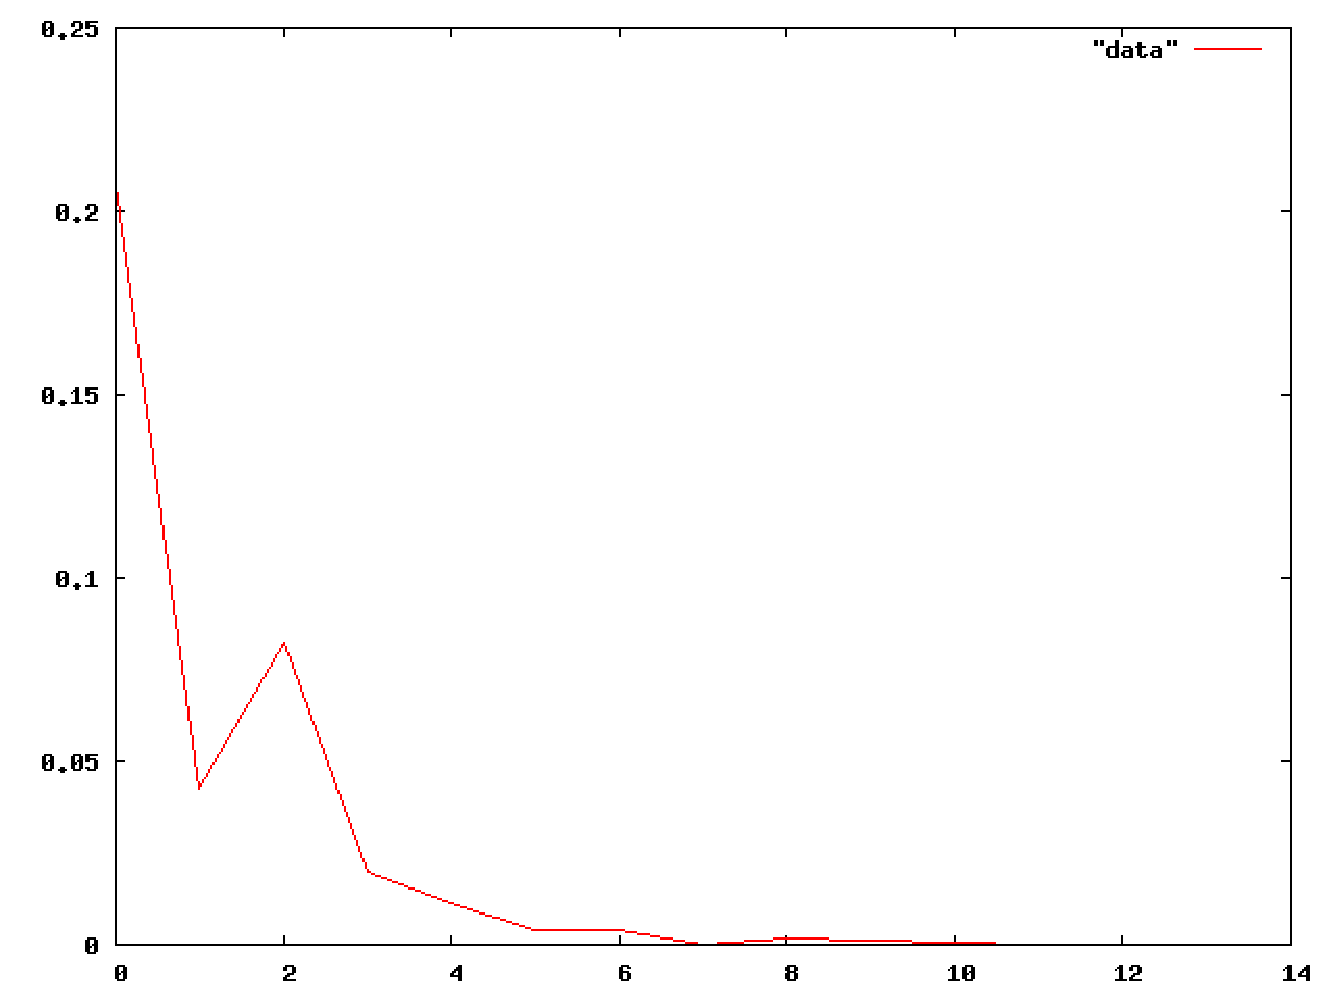
\includegraphics[width=0.7\textwidth]{./images/grafico}
\end{figure}


%%%%%%%%%%%%%%%%%%%%%

\subsection*{Note sui cicli}

Il codice proposto al \emph{Punto 1} utilizza un ciclo \cpp{while}.
%Un' altra alternativa possibile \`e l'uso di un ciclo \texttt{while}:
%\lstset{basicstyle=\scriptsize\sf}
%\lstinputlisting[caption=Ciclo \texttt{while} senza
%\texttt{break}.,linerange={26-47}]{es/1/zerofun-while.cc}
%\lstset{basicstyle=\sf}
In queso caso la prima valutazione della funzione \`e necessariamente esterna
al ciclo.

In alternativa si potrebbe scrivere un ciclo \cpp{for} ed utilizzare
l'istruzione \texttt{break} qualora venisse raggiunta la convergenza entro
il massimo numero di iterazioni.
\lstset{basicstyle=\scriptsize\sf}
    \lstinputlisting[caption=Ciclo \texttt{for} con
        \texttt{break}.,linerange={26-67}]{es/1/old_file/zerofun-break.cc}
\lstset{basicstyle=\sf}
L'istruzione \texttt{break} \`e un modo efficiente per
imporre una condizione di uscita, ma pu\`o rendere il codice di difficile
lettura ed interpretazione; infatti le condizioni di uscita sono sparse e non
sono raggruppate all'inizio o alla fine. Per questo motivo si cerca di limitare
l'uso di \texttt{break} alla gestione di eccezioni.

Una soluzione alternativa \`e basata sul ciclo \cpp{do}/\cpp{while}:
\lstset{basicstyle=\scriptsize\sf}
\lstinputlisting[caption=Ciclo \texttt{do\ldots while} senza
    \texttt{break}.,linerange={26-47}]{es/1/old_file/zerofun-dowhile.cc}
\lstset{basicstyle=\sf}
In questo caso le condizioni di uscita sono chiaramente visibili in fondo al
codice. Il prezzo da pagare \`e un inutile assegnamento di variabili
nell'ultima iterazione eseguita. Il costrutto \texttt{do \ldots while} ha come
caratteristica fondamentale quella di eseguire sempre almeno una iterazione,
anche se le condizioni di uscita non sono verificate o
verificabili all'inzio del ciclo.
A volte questo comportamento pu\`o aiutare a generare errori non banali,
se il codice scritto \`e complesso.



\bibliographystyle{siam}
\bibliography{../common/bibliography}

\end{document}
